\documentclass[fontsize=12pt, a4paper, headinclude, twoside=false, parskip=half+, pagesize=auto, numbers=noenddot, plainheadsepline, open=right, toc=listof, toc=bibliography, chapteratlists=0pt]{scrreprt}

%\usepackage{calc}
%\usepackage[a4paper,textwidth=\textwidth]{geometry}
%\addtolength{\paperwidth}{6cm}
%\addtolength{\marginparwidth}{6cm}


% Allgemeines
\usepackage[automark]{scrpage2} % Kopf- und Fußzeilen
\usepackage{amsmath,marvosym} % Mathesachen
\usepackage[T1]{fontenc} % Ligaturen, richtige Umlaute im PDF
\usepackage[utf8]{inputenc}% UTF8-Kodierung für Umlaute usw
%\usepackage{perpage} %the perpage package
%\MakePerPage{footnote} %the perpage package command
\usepackage{caption}
\usepackage[Q=yes]{examplep}
\usepackage[colorinlistoftodos]{todonotes}

% Schriften
\usepackage{setspace} % Zeilenabstand
\onehalfspacing % 1,5 Zeilen
\usepackage{lmodern}

% Schriften-Größen
\setkomafont{chapter}{\Huge\rmfamily} % Überschrift der Ebene
\setkomafont{section}{\Large\rmfamily}
\setkomafont{subsection}{\large\rmfamily}
\setkomafont{subsubsection}{\small\rmfamily}
\setkomafont{chapterentry}{\large\rmfamily} % Überschrift der Ebene in Inhaltsverzeichnis
\setkomafont{descriptionlabel}{\bfseries\rmfamily} % für description Umgebungen
\setkomafont{captionlabel}{\small\bfseries}
\setkomafont{caption}{\small}

% Custom colors
\definecolor{deepblue}{rgb}{0,0,0.5}
\definecolor{deepred}{rgb}{0.6,0,0}
\definecolor{deepgreen}{rgb}{0,0.5,0}
\definecolor{grau}{rgb}{0.5,0.5,0.5}

% Sprache: Deutsch
\usepackage[ngerman]{babel} % Silbentrennung

% PDF
\usepackage[ngerman, breaklinks=true]{hyperref}
\usepackage[final]{microtype} % mikrotypographische Optimierungen
\usepackage{url}
\usepackage{pdflscape} % einzelne Seiten drehen können

% Tabellen
\usepackage{multirow} % Tabellen-Zellen über mehrere Zeilen
\usepackage{multicol} % mehre Spalten auf eine Seite
\usepackage{tabularx} % Für Tabellen mit vorgegeben Größen
\usepackage{longtable} % Tabellen über mehrere Seiten
\usepackage{array}
\usepackage{float}
\usepackage{booktabs}

% Diagramme
%\usepackage{tikz}
%\usepackage{pgfplotstable}
%\usepackage{pgfplots}
%\usetikzlibrary{trees}

%  Bibliographie
\usepackage{bibgerm} % Umlaute in BibTeX
\usepackage{cite}
%% For changing the IEEE citation style
\makeatletter
\def\bstctlcite{\@ifnextchar[{\@bstctlcite}{\@bstctlcite[@auxout]}}
\def\@bstctlcite[#1]#2{\@bsphack
	\@for\@citeb:=#2\do{%
		\edef\@citeb{\expandafter\@firstofone\@citeb}%
		\if@filesw\immediate\write\csname #1\endcsname{\string\citation{\@citeb}}\fi}%
	\@esphack}
\makeatother


% Bilder
\usepackage{graphicx} % Bilder
\graphicspath{{images/}}
\DeclareGraphicsExtensions{.pdf,.png,.jpg} % bevorzuge pdf-Dateien
\usepackage[all]{hypcap} % Beim Klicken auf Links zum Bild und nicht zu Caption gehen


% Bildunterschrift
\usepackage{caption}
\usepackage{chngcntr}
\counterwithout{figure}{chapter}
\setcapindent{0em} % kein Einrücken der Caption von Figures und Tabellen
\setcapwidth[c]{0.9\textwidth}
\setlength{\abovecaptionskip}{0.2cm} % Abstand der zwischen Bild- und Bildunterschrift

% Quellcode
\usepackage{listings} % für Formatierung in Quelltexten

% Default fixed font does not support bold face
\DeclareFixedFont{\ttb}{T1}{txtt}{bx}{n}{10} % for bold
\DeclareFixedFont{\ttm}{T1}{txtt}{m}{n}{10}  % for normal

\lstset{
    extendedchars=true,
	numberbychapter=true,
	basicstyle=\scriptsize\ttm,
 	frame=l,
	captionpos=b,		
	xleftmargin=5pt,
	tabsize=2,
    numbers=none,
	numberstyle=\scriptsize,
	numbersep=10pt,
	breakautoindent  = true,
	breaklines       = true,
	breakatwhitespace = true,
	prebreak=\raisebox{0ex}[0ex][0ex]{\ensuremath{\hookleftarrow}}
}


% Python environment
\lstnewenvironment{python}[2][]
{
\vspace{10pt}
\lstset{
    caption=#1,
    label=lst.#2,
	language=Python,
	commentstyle=\color{grau},
	morekeywords={self}, % Add keywords here
	deletekeywords=[2]{help}, 
	keywordstyle=\ttb\color{deepblue},
	stringstyle=\color{deepgreen},
	showstringspaces=false,
	}
}
{}


% typearea berechnet einen sinnvollen Satzspiegel (das heißt die Seitenränder) siehe auch http://www.ctan.org/pkg/typearea. Diese Berechnung befindet sich am Schluss, damit die Einstellungen oben berücksichtigt werden
%\typearea{14} 



% Eigene Befehle %%%%%%%%%%%%%%%%%%%%%%%%%%%%%%%%%%%%%%%%%%%%%%%%%
\newcommand{\image}[4][!h]{
	\begin{figure}[#1]
		\centering
		\vspace{1ex}
		\includegraphics[#3]{images/#2}
		\caption[#4]{#4}\label{img.#2}      
		\vspace{1ex}
	\end{figure}
}

 % Importiere die Einstellungen aus der Präambel

\begin{document} % hier beginnt der eigentliche Inhalt
\bstctlcite{IEEE:BSTcontrol} % Fix für Zitatstyle
\pagenumbering{Roman} % große Römische Seitenummerierung
\pagestyle{empty}

% Titelseite
%\clearscrheadings\clearscrplain

\begin{center}

\begin{Huge} 
Hochschule für Studiengänge \\
\end{Huge}

\begin{Large}
Fakultät für Sachen und Dinge \\
\end{Large}

\vspace{20mm}

\begin{Large}
[TITEL]

\vspace{2cm}
 
[ENGLISCHER TITEL]

\end{Large}



\vspace{1cm}

MASTERARBEIT\\

\vspace{4.5cm}

[NAME] \\
Matrikel-Nummer 1111111 \\

\vspace{4cm}

Prüfer: Prof. Dr. Chris P. Bacon\\


\end{center}
\clearpage

\pagestyle{useheadings} % normale Kopf- und Fußzeilen für den Rest

\chapter*{Erklärung}
Hiermit erkläre ich, dass ich die Masterarbeit selbständig verfasst, noch nicht anderweitig für Prüfungszwecke vorgelegt, keine anderen als die angegebenen Quellen oder Hilfsmittel benutzt sowie wörtliche und sinngemäße Zitate als solche gekennzeichnet habe.
\vspace{3cm}

Ort, Datum \hspace{5cm} Unterschrift

\chapter*{Zusammenfassung}

In dieser Masterarbeit wird erforscht welche Auswirkungen Bla und Blubb auf Dinge haben.

\listoftodos

\tableofcontents % Inhalt


\chapter{Auflistung}
\pagenumbering{arabic} % ab jetzt die normale arabische Nummerierung


\begin{itemize}
	\item[-] bla
	\item[-] blubb
	\item[-] usw
\end{itemize}


\chapter{Zitate}
Behauptung und Quelle. \cite{google}
\todo{Mehr Quellen}
\missingfigure{hier muss noch ein Bild rein }

\chapter{Bilder}

\image{useCase}{scale=.9}{Anwendungsfalldiagramm}

\chapter{Codelistings}



\begin{python}[Starten einer Suche in DomainSearch.py]{suchstart}
	def perform_search(name):
	with threading.Lock():
	# Perform one search for the given domain.
	name = name.strip()
	out.print_search_started(name)
	
	db = database.db()
	searchID = db.insert_search(name)
	db.close_connection()
	
	sched = scheduler.Scheduler()
	sched.find_modules()
	sched.start_modules(searchID, name)
\end{python}


\vspace{6mm}
\begin{lstlisting}[caption=DNS Auflösung von cs.hm.edu, label=lst.dnsDig, ]
cs.hm.edu.	1800	IN	NS	ns.e-technik.fh-muenchen.de.
cs.hm.edu.	1800	IN	NS	ns.hm.edu.
cs.hm.edu.	72791	IN	A   129.187.244.60
cs.hm.edu.	14260	IN	MX	10 mailrelay2.lrz.de.
cs.hm.edu.	14260	IN	MX	10 mailrelay1.lrz.de.
\end{lstlisting}


\chapter{Tabellen}

\begin{table}
	\begin{center}
		\begin{tabular}{ l c }
			\toprule
			\textbf{Modul} & \textbf{Durchschnittslaufzeit in Sekunden}\\
			\midrule   
			DNSresolver            & 0,314 \\
			DomainAge               & 0,495 \\
			GeoIP                   & 2,195 \\
			GoogleSafeBrowsingAPI   & 0,145 \\
			GoogleSearch            & 1,349 \\
			Nmap                    & 4,836 \\
			RobotsTxt               & 0,284 \\
			Traceroute              & 10,026 \\
			Typo                    & 0,583 \\
			Whois                   & 0,166 \\
			\midrule
			\textbf{Alle Module}    & \textbf{10,043} \\
			\bottomrule
		\end{tabular}
		\caption{Laufzeiten der einzelnen Module}\label{tab.laufzeit}
	\end{center}
\end{table}


\begin{figure}[!hbt]
	\begin{minipage}[!hbt]{5cm}
		\centering
		
		\begin{tabular}{ l  c }
			\toprule
			\textbf{Anzahl Threads} & \textbf{Laufzeit}\\
			& \textbf{in Sekunden}\\
			\midrule
			Sequenziell             & 531,27 \\
			2                       & 260,67 \\
			5                       & 106,77 \\
			10                      & 69,02 \\
			15                      & 70,53 \\
			20                      & 66,48 \\
			50                      & 62,94 \\
			\bottomrule
		\end{tabular}
		
	\end{minipage}
	\hfill
	\begin{minipage}[!hbt]{8.2cm}
		\centering
	
		
			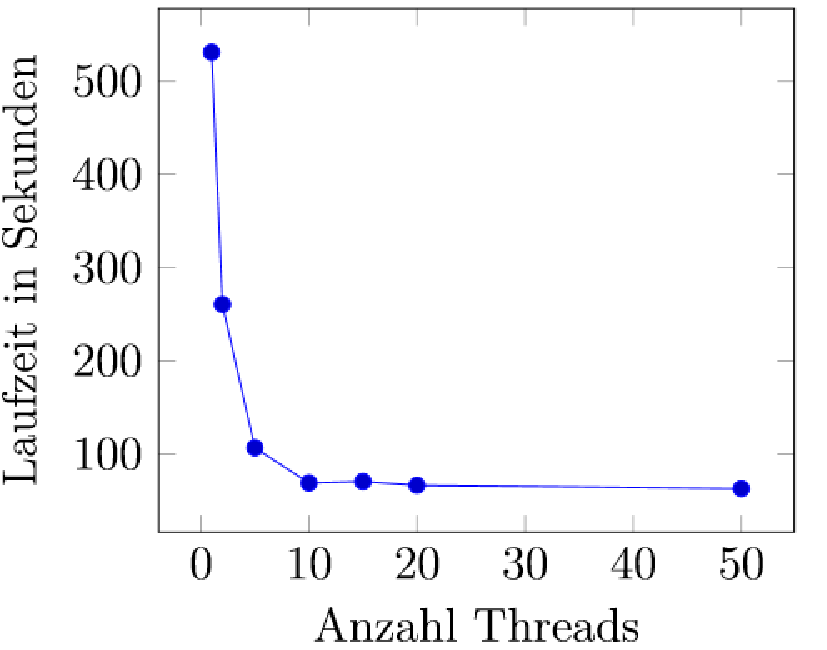
\includegraphics[scale=0.6]{images/laufzeiten}			 
		
	\end{minipage}
	\caption{Anzahl der Threads im Verhältnis zu Laufzeit}\label{fig.laufzeitListe}
\end{figure}



\listoffigures
\lstlistoflistings
\listoftables

\bibliographystyle{ieeetran}
\bibliography{bibliographie}

\end{document}
